\chapter{Proposal}\label{chap:40}
In alignment with the objectives delineated in Section \ref{10:spec-obj}, this chapter presents the newly proposed architectural framework termed \textbf{CA-BiFPN}. This design draws inspiration from the \textit{two-stage detector} paradigm, as comprehensively elucidated in Chapter \ref{chap:related-work}. The architecture is strategically segmented into three primary components:
\begin{enumerate}
    \item \textbf{Backbone}: This component represents the refined network specifically tailored for feature extraction. Within this segment, we harness feature maps from diverse stages of the network. The intent is to meticulously capture feature maps both from advanced (high-level) stages and foundational (low-level) stages of the network.
    \item \textbf{Neck}: The \textit{neck} merges connections from various stages of the backbone. It incorporates the structure of the \textit{BiFPN}~\cite{DBLP:journals/corr/abs-1911-09070}. Within this framework, we introduced two new components: the \textbf{Local Context Aggregator} and the \textbf{Global Context Aggregator}. A deeper exploration of these components will be provided in Section \ref{sec:cau}.
    \item \textbf{Head Detector}: This segment integrates a \textit{Mask R-CNN} head~\cite{DBLP:journals/corr/HeGDG17}, equipped with two distinct \textit{RoI Pooler} operators. While one is dedicated to the Object Detection task, the other is tailored for the Instance Segmentation task. These poolers subsequently receive inputs from the varied fused levels extended by the \textit{neck}.
\end{enumerate}
A comprehensive visualization of the final architecture is presented in Figure \ref{fig:40:arq-ca-bifpn}.\\
\begin{figure}[htb]
    \centering
    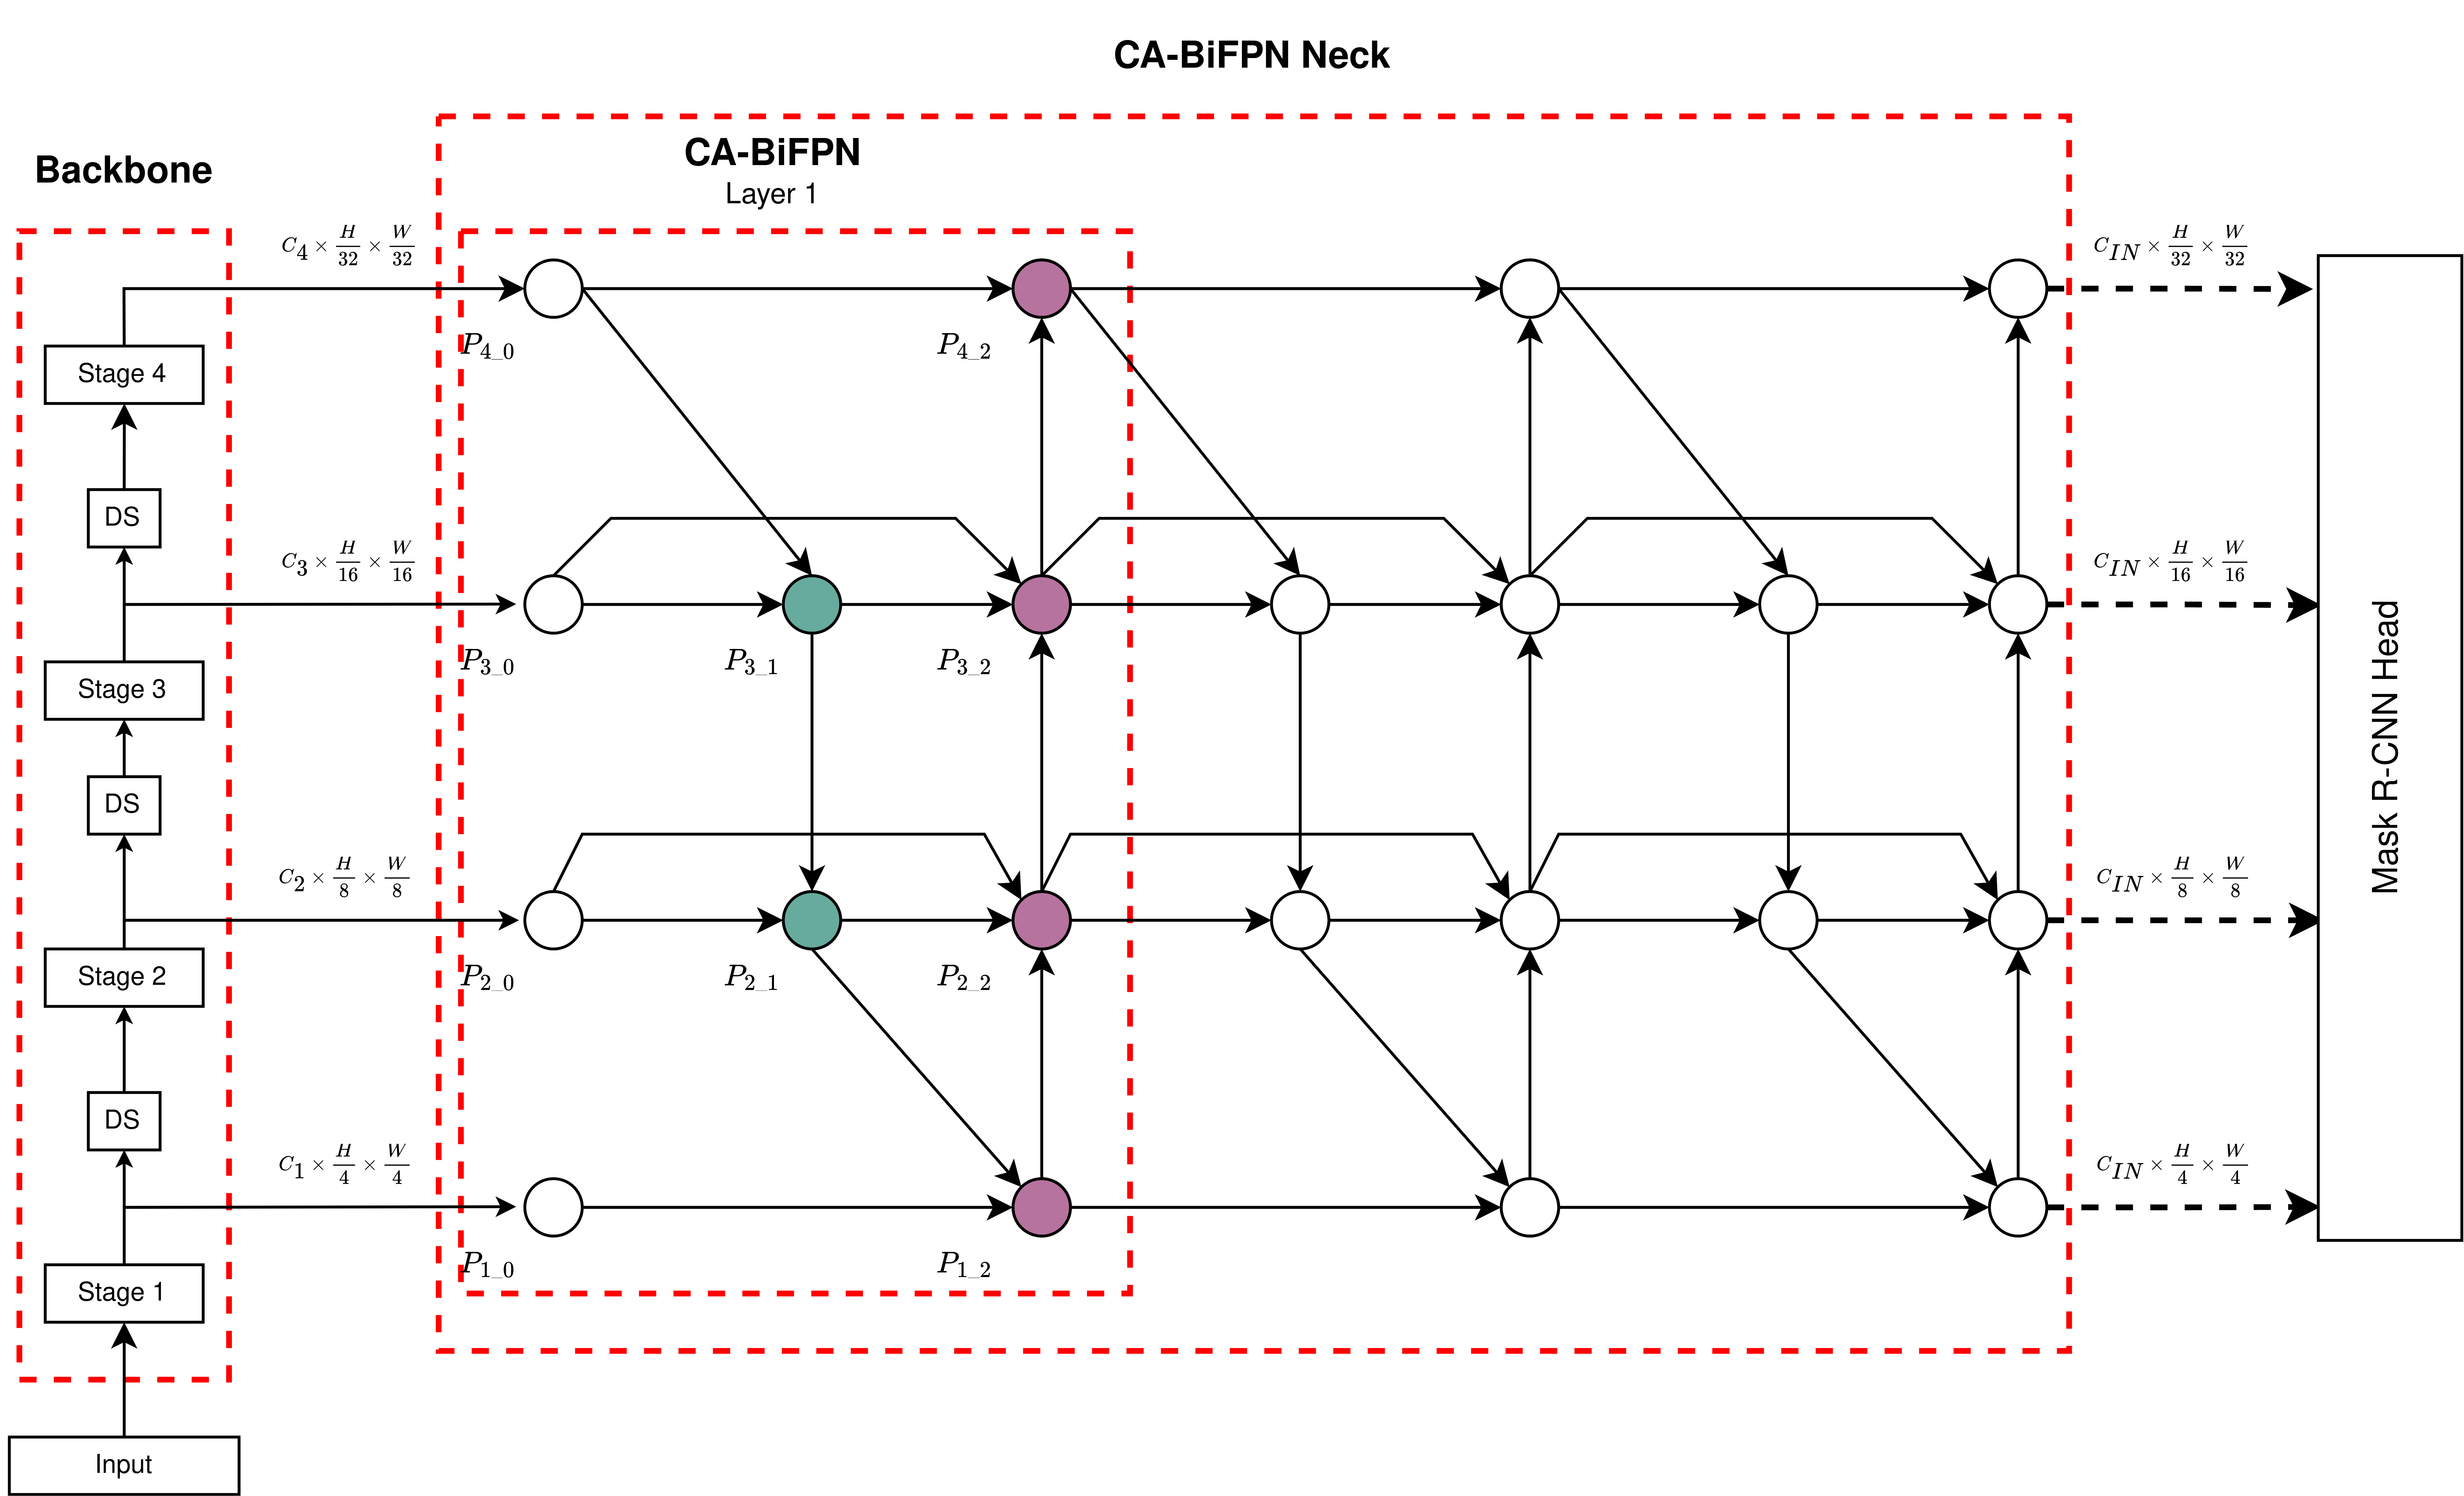
\includegraphics[width=1\linewidth]{figures/chapters-imgs/40/arq-ca-bifpn.jpg}
    \caption[Detailed schematic of the CA-BiFPN architecture]{Detailed schematic of the CA-BiFPN architecture.}
    \label{fig:40:arq-ca-bifpn}
\end{figure}

The subsequent sections will delve into the design intricacies of the \textit{Context Aggregator Units} located within the \textit{neck}, emphasizing their integration within the \textit{BiFPN} structure.

\section{Context Aggregator Units} \label{sec:cau}
Drawing parallels with \textit{ParseNet}~\cite{DBLP:journals/corr/LiuRB15}, the \textit{Context Aggregator} unit is designed to synergize both local and global features emanating from the backbone stage. Within the scope of this research, the distinctions between local and global contextual features are articulated as follows:
\begin{enumerate}
    \item \textbf{Local Context Feature}: These originate from the deeper stage layers in the backbone, often referred to as the bottom-up pathway of the network. Possessing a minimal receptive field, these features preserve intricate spatial information, thereby facilitating the generation of high-level features.
    \item \textbf{Global Context Feature}: The features extracted from the shallower stages of the backbone, characterized by their expansive receptive field, are adept at capturing robust semantic information. These are categorized as low-level features.
\end{enumerate}

\subsection{Global Context Operator}
In the \textit{Squeeze-and-Excitation} networks study~\cite{DBLP:journals/corr/abs-1709-01507}, the convolutional vector operation presented in Equation (\ref{eq:conv:layer}), denoted as $\boldsymbol{K}*\boldsymbol{x}$, involves a summation across all channels \( C \). The output from this operation is closely interwoven with the local spatial correlations captured by the filters \( \boldsymbol{K} \).
To address the convolutional complexities, the squeeze-and-excitation block integrates global spatial information throughout the channels and subsequently consolidates this data through channel-wise dependencies. Then, for an input \( \mathbf{X} \in \mathbb{R}^{C \times H \times W} \), the \textit{global feature context operator} of the squeeze-and-excitation block is defined as follows:
\begin{equation}
\mathbf{G}(\mathbf{X})=\mathbf{W}_2\left(\delta\left(\mathbf{W}_1(\mathbf{g}(\mathbf{X}))\right)\right),
\end{equation}
where both \(\mathbf{W}_1 \in \mathbb{R}^{\frac{C}{r} \times C}\) and \(\mathbf{W}_2 \in \mathbb{R}^{C \times \frac{C}{r}}\) represent learnable weights. The channel reduction factor is denoted as \(r\) and usually takes values within the set \(\{2,4\}\). Here, \(\delta\) signifies the activation function. The squeeze operator, symbolized as \(\mathbf{g}(\mathbf{X})\), is formulated as:
\begin{equation}
g(\mathbf{X})_c=\frac{1}{H \times W} \sum_{i=1}^H \sum_{j=1}^W x_{c,i,j}.
\end{equation}
In this equation, \(g(\mathbf{X})_c\) is a component of \(\mathbf{g}(\mathbf{X}) \in \mathbb{R}^{C}\), and \(x_{c,i,j}\) corresponds to individual units of the feature map \(\mathbf{X}\).\\

Building upon the concept of point-wise channel representation introduced by the \textit{global feature context operator}, we focus on the interaction of the global spatial information throughout the channels. This approach mirrors that of the \textit{MS-CAM} block presented by \textit{Yimian Dai et al.} in their research titled \textit{Attentional Feature Fusion}~\cite{DBLP:journals/corr/abs-2009-14082}. Guided by their insights, we have chosen to implement the \textit{point-wise convolution} for channel aggregation, specifically targeting the learnable weights \( \mathbf{W}_1 \) and \( \mathbf{W}_2 \). 

As a result, the \textbf{Global Context Operator} formulated in our study can be expressed through the following equation:

\begin{equation}
\sigma\left(\mathbf{G}(\mathbf{X})\right) = \sigma\left(\operatorname{PW-Conv_{1\times 1}}\left(\delta\left(\operatorname{PW-Conv_{1\times 1}}(\mathbf{g}(\mathbf{X}))\right)\right)\right). \label{eq:block-GCA}
\end{equation}

Within this equation, \( \sigma \) denotes the \textit{Sigmoid} function, while \( \delta \) refers to the GELU~\cite{hendrycks2023gaussian} activation function. The term \( \operatorname{PW-Conv_{1\times 1}} \) signifies the point-wise convolution. Following this, a channel-wise multiplication is performed between the output \( \sigma\left(\mathbf{G}(\mathbf{X})\right) \) and the input \( \mathbf{X} \). A graphical representation of the \textbf{Global Context Operator} is available in Figure \ref{fig:40:block-GCA}.

\begin{figure}[htb]
    \centering % <-- added
\begin{subfigure}{0.3\textwidth}
  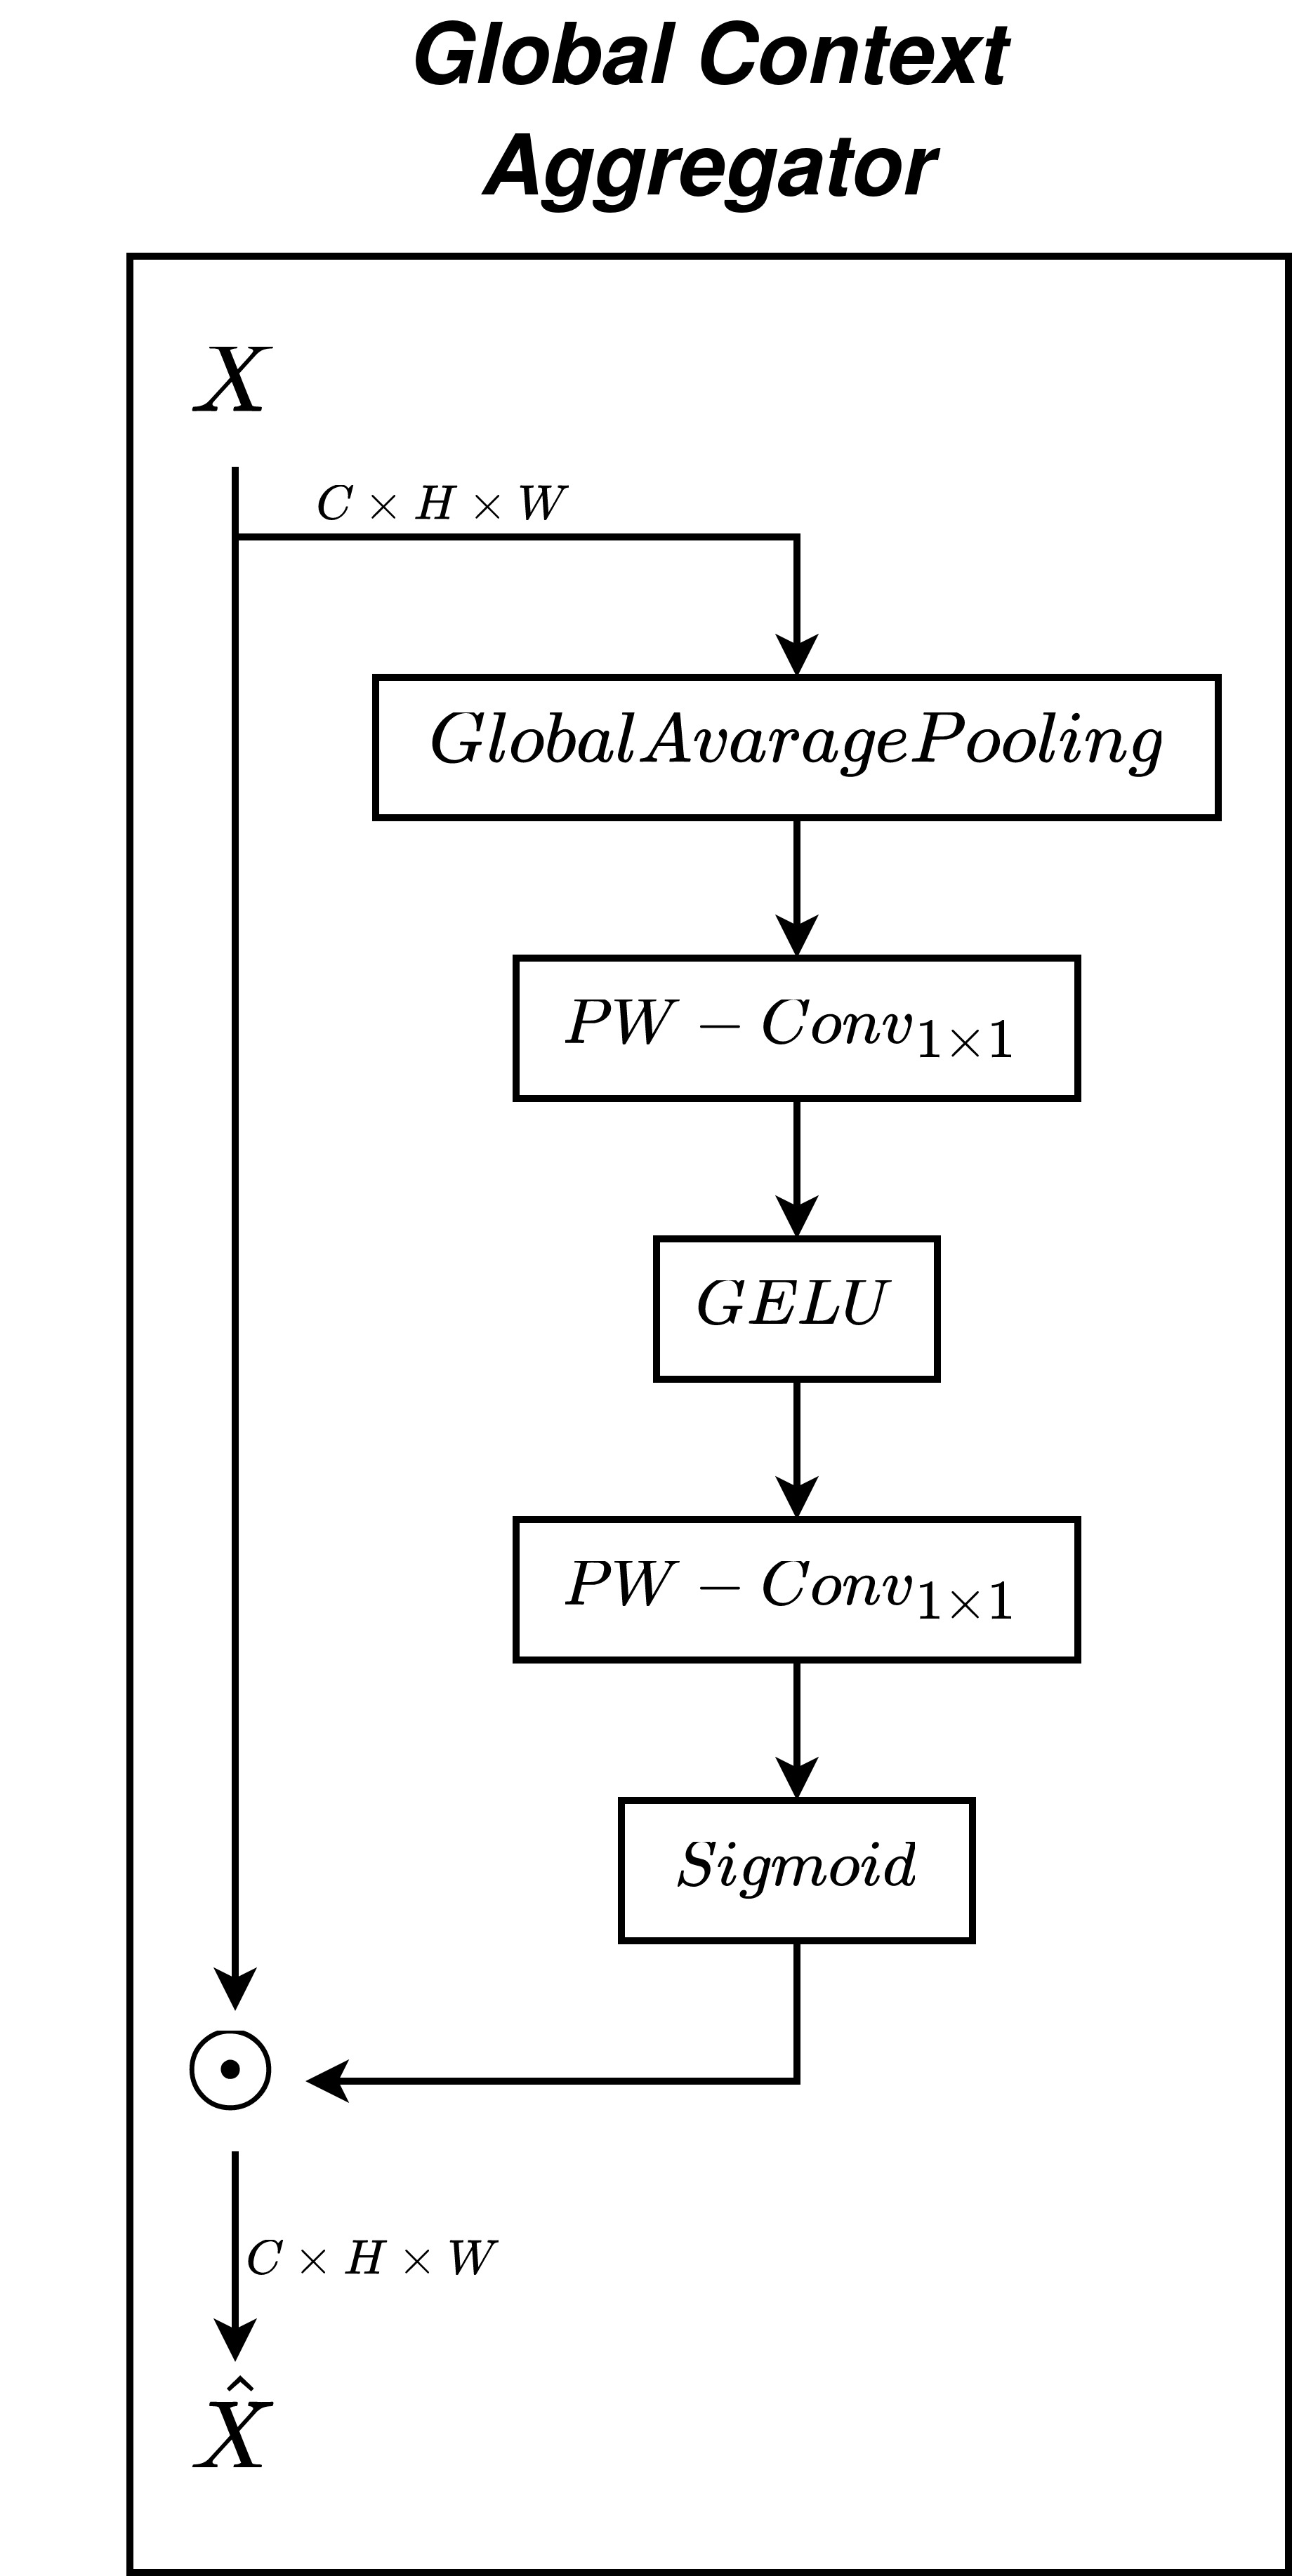
\includegraphics[width=\linewidth]{figures/chapters-imgs/40/block-GCA.jpg}
  \caption{\protect\raggedright Detailed schematic Global Context Aggregator Unit.}
  \label{fig:40:block-GCA}
\end{subfigure} % <-- added
% \medskip
\hspace{3mm}
\begin{subfigure}{0.3\textwidth}
  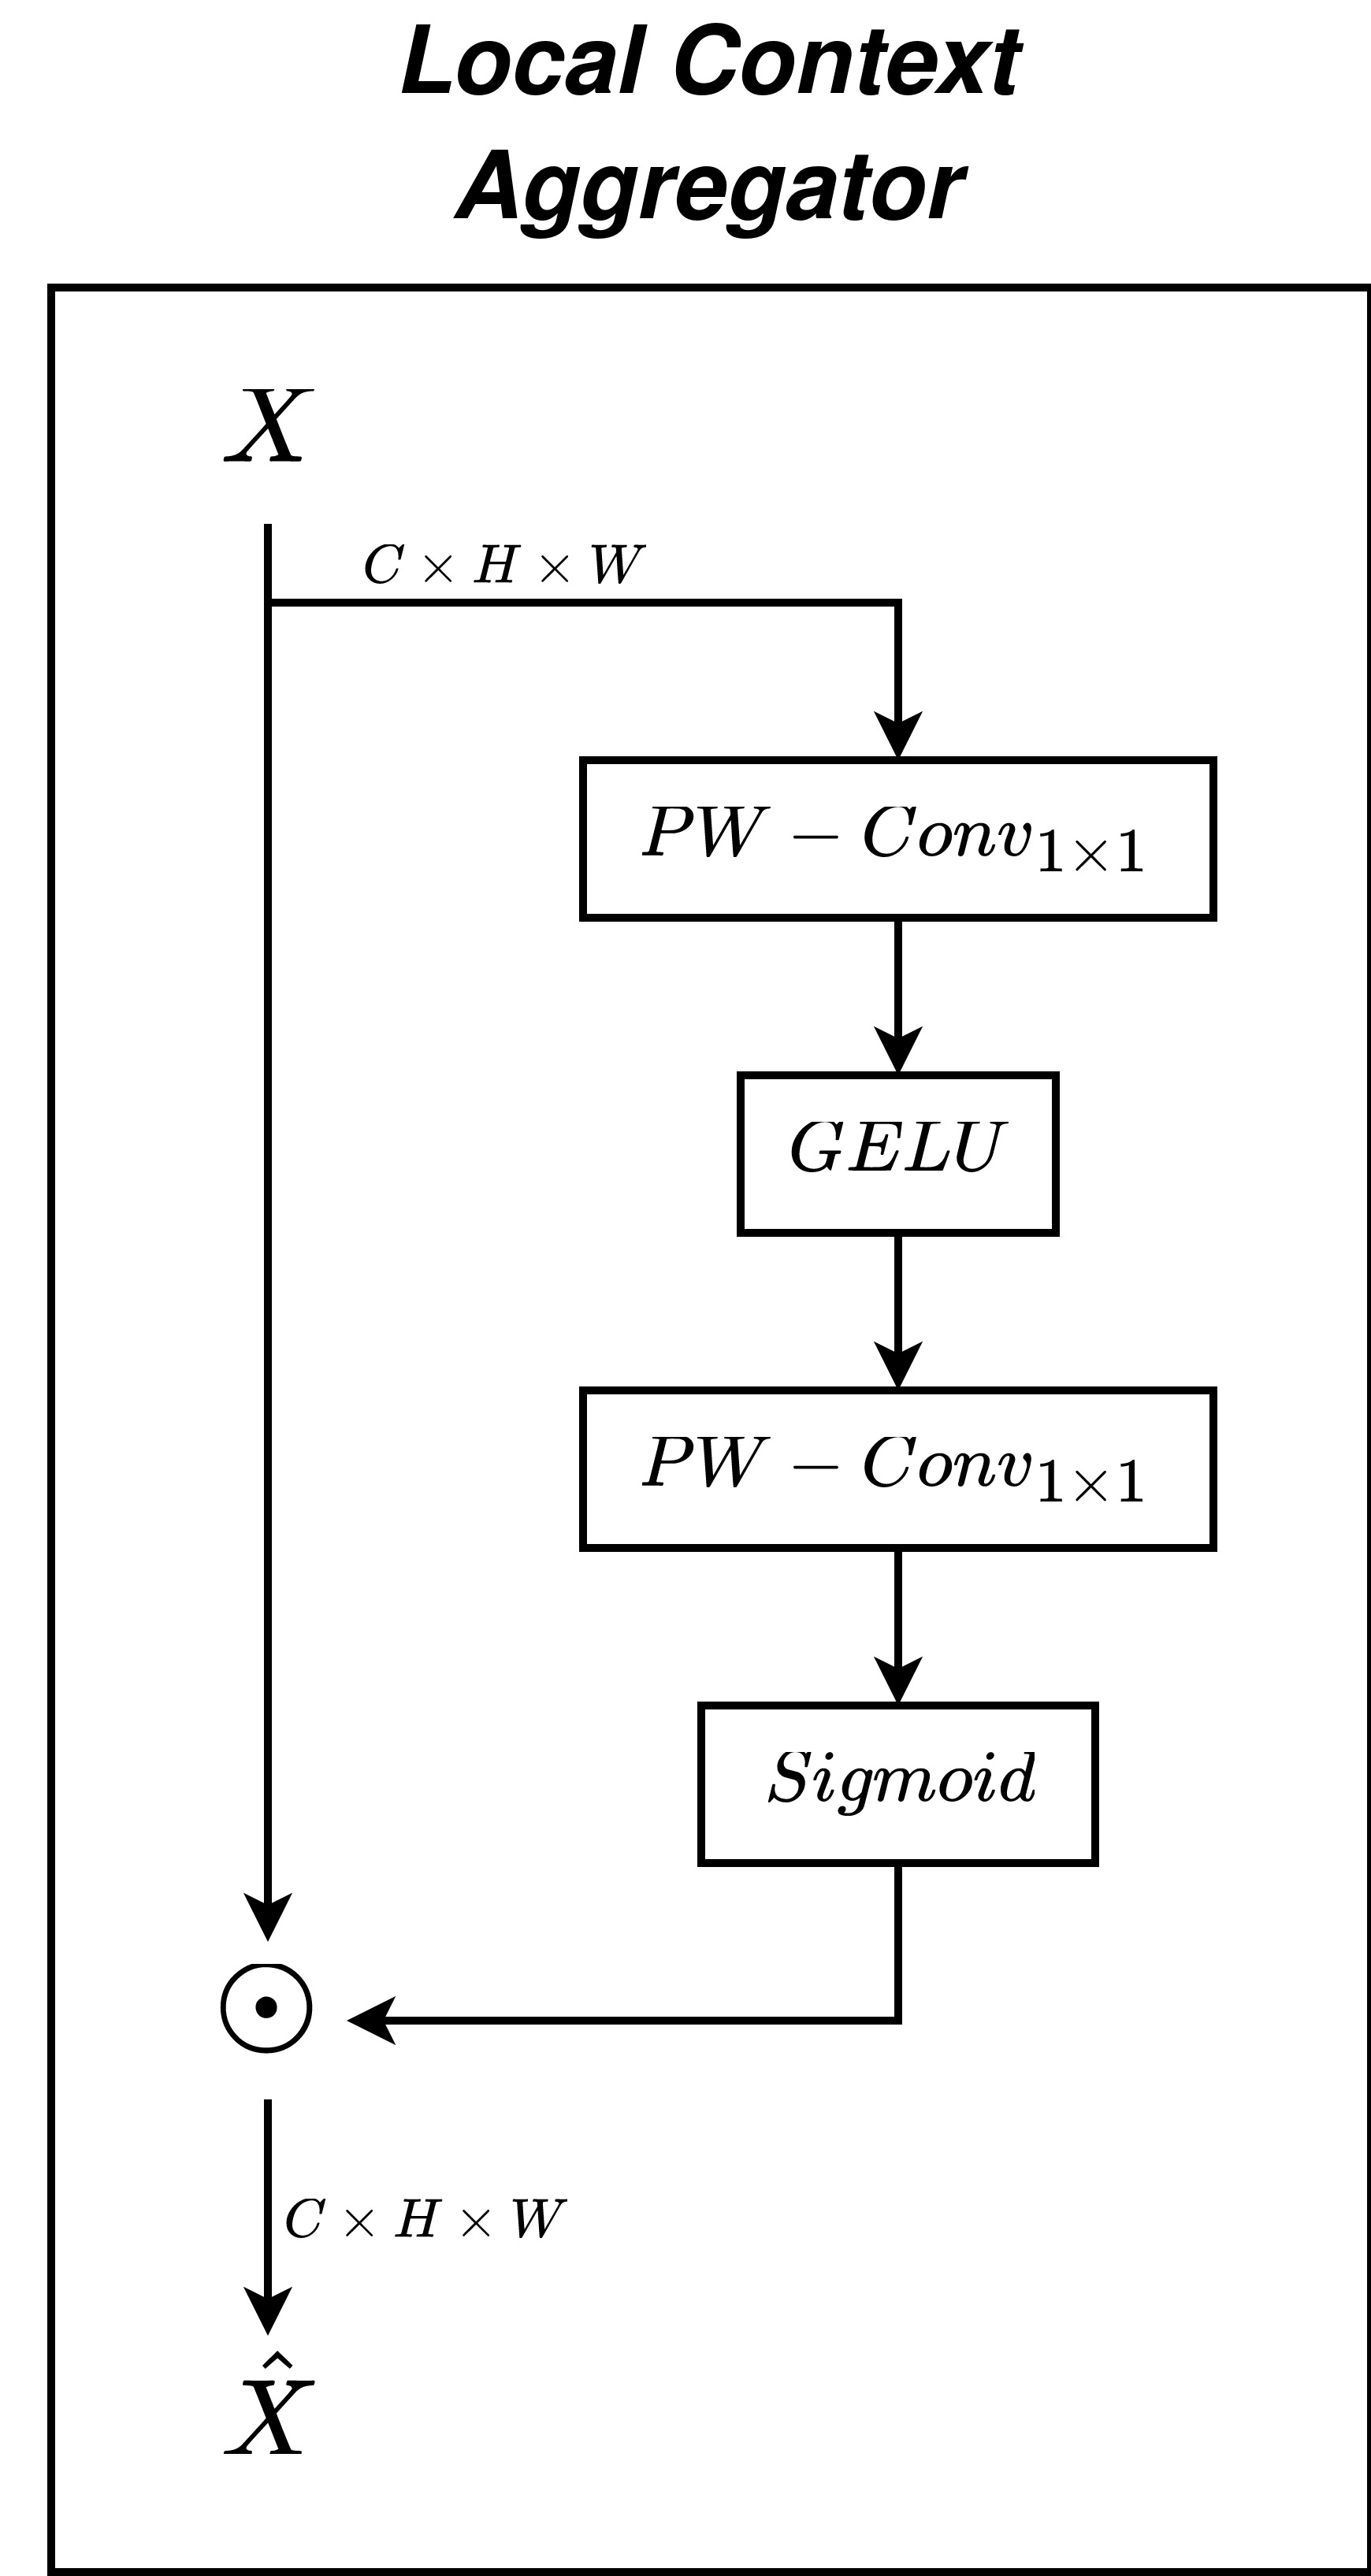
\includegraphics[width=\linewidth]{figures/chapters-imgs/40/block-LCA.jpg}
  \caption{\protect\raggedright Detailed schematic Local Context Aggregator Unit.}
  \label{fig:40:block-LCA}
\end{subfigure}
% \medskip
\hspace{3mm}
\begin{subfigure}{0.3\textwidth}
  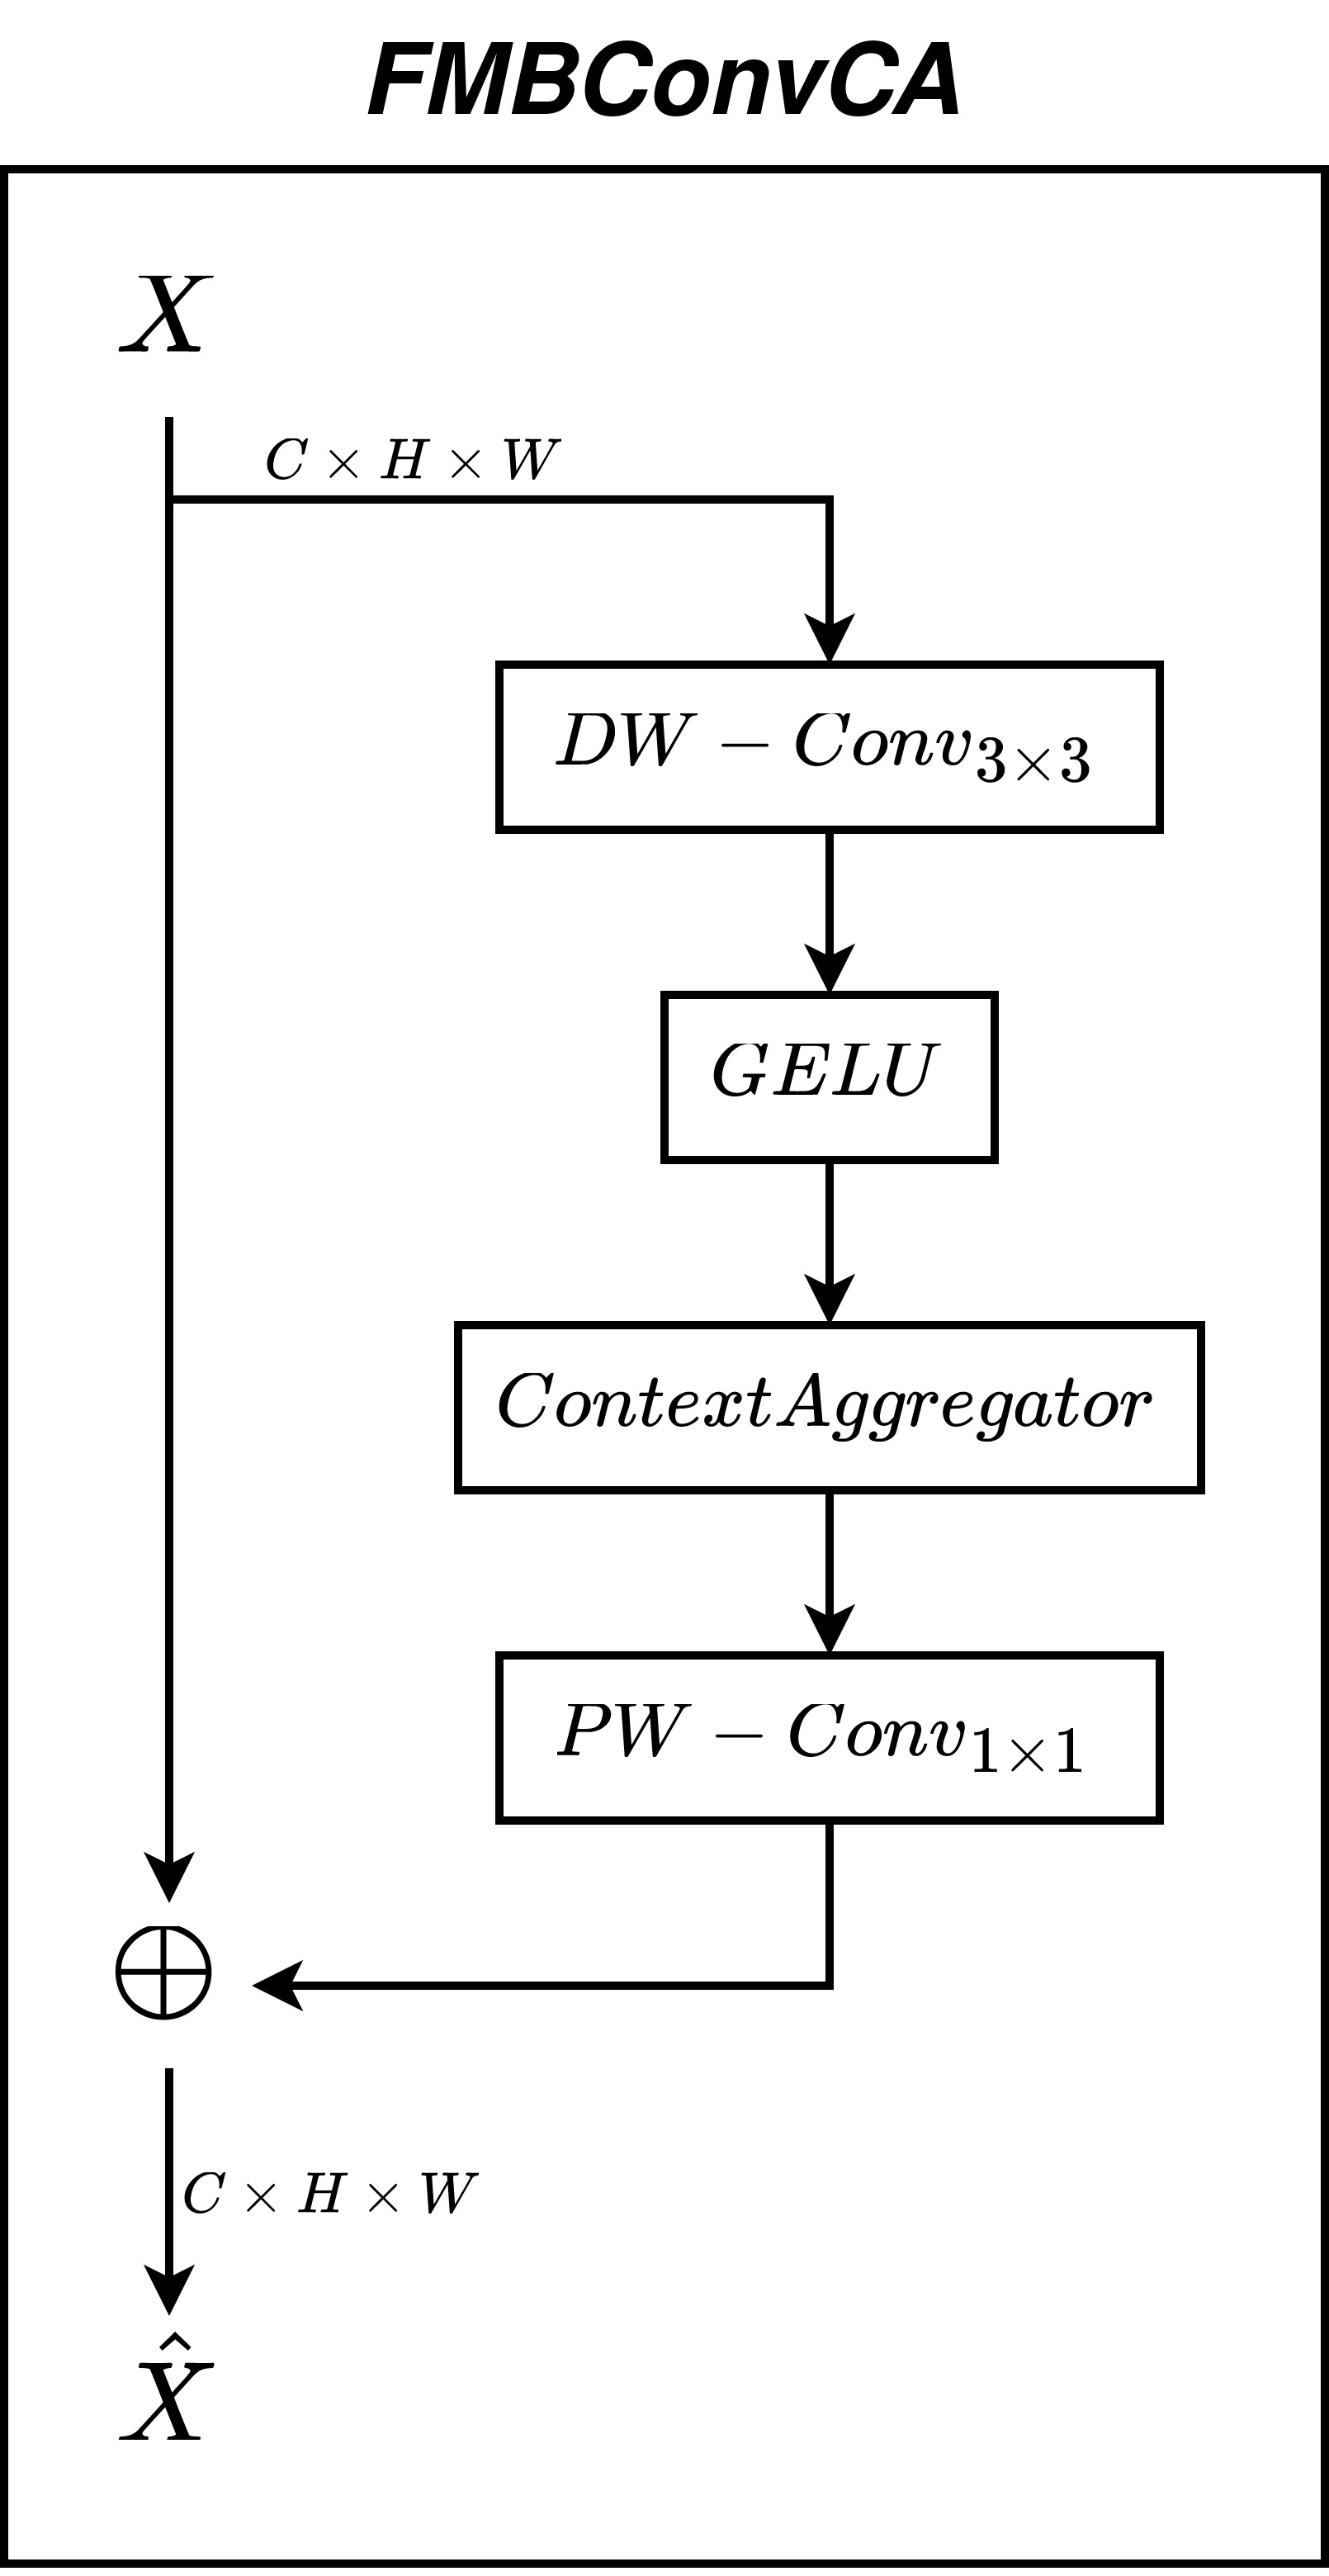
\includegraphics[width=\linewidth]{figures/chapters-imgs/40/block-FMBC.jpg}
  \caption{\protect\raggedright Detailed schematic of the merge unit node.}
  \label{fig:40:block-FMBC}
\end{subfigure}

\caption{Diagram illustrating the Context Aggregator Units and merge unit node FMBConvCA, proposed in this work.}
\end{figure}

\subsection{Local Context Operator}
Given the understanding that channel relationships shaped by convolution are inherently implicit and localized, the \textit{Local Context Operator} functions as a simplified version of equation (\ref{eq:block-GCA}). Notably, this operator excludes the \textit{global feature context operator}:

\begin{equation}
\sigma\left(\mathbf{L}(\mathbf{X})\right) = \sigma\left(\operatorname{PW-Conv_{1\times 1}}\left(\delta\left(\operatorname{PW-Conv_{1\times 1}}(\mathbf{X})\right)\right)\right). \label{eq:block-LCA}
\end{equation}

Mirroring the process in equation (\ref{eq:block-GCA}), a channel-wise multiplication is carried out between the output \( \sigma\left(\mathbf{L}(\mathbf{X})\right) \) and the input \( \mathbf{X} \). A graphical illustration of the \textbf{Local Context Operator} can be found in Figure \ref{fig:40:block-LCA}.

\subsection{FMBConvCA Block}
After establishing the architecture of the \textit{Context Aggregator Units}, we incorporate them into a refined version of the \textit{Fused-MBConv} block~\cite{Gupta_Tan2019}, hereafter referred to as \textbf{FMBConvCA}. This modification is analogous to the enhanced block delineated in the study by \textit{Hatamizadeh et al.}~\cite{hatamizadeh2023global}. The purpose of this novel block is to imbue the network with advantageous characteristics, such as inductive bias and the capacity to model inter-channel dependencies, particularly at the various stages within the neck of the architecture.
The bottleneck equation for the \textit{FMBConvCA} block can be formally defined as follows: 

\begin{equation}
\operatorname{FMBConvCA}\left(\mathbf{X}\right) = \operatorname{PW-Conv_{1\times 1}}\left(\operatorname{CA}\left(\delta\left(\operatorname{DW-Conv_{3\times 3}}\left(\mathbf{X}\right)\right)\right)\right), \label{eq:block-FMBC}
\end{equation}

In Equation \ref{eq:block-FMBC}, the term \( \operatorname{DW-Conv_{3\times 3}} \) denotes a \( 3 \times 3 \) depth-wise convolution operation~\cite{DBLP:journals/corr/abs-1709-01507}. The symbol \( \delta \) is employed to represent the Gaussian Error Linear Unit (GELU) activation function~\cite{hendrycks2023gaussian}. Moreover, \( \operatorname{PW-Conv_{1\times 1}} \) signifies the point-wise convolution operation. Within this equation, \( \operatorname{CA} \) stands for the \textit{Context Aggregator Units}, which can take the form of either \( \sigma\left(\mathbf{L}(\mathbf{X})\right) \) or \( \sigma\left(\mathbf{G}(\mathbf{X})\right) \). Lastly, the output of the \(\operatorname{FMBConvCA}\left(\mathbf{X}\right)\) operation is subject to direct summation with the input vector \( \mathbf{X} \).
A visual representation of the \(\operatorname{FMBConvCA}\) block is provided in Figure \ref{fig:40:block-FMBC}.\\

The incorporation of the \textit{Context Aggregator Units} into the \textbf{FMBConvCA} block provides enhanced capabilities for contextual understanding and feature extraction. By elegantly combining the depth-wise and point-wise convolutions with the \textit{Context Aggregator Units} and GELU activation function, the block aims to achieve a balance between computational efficiency and representational power. This design fosters a robust architecture capable of handling intricate data patterns and inter-channel dependencies, thereby amplifying the overall performance of the neck.

\section{Architecture of the CA-BIFPN Neck} \label{sec:cabifpn-neck}
As alluded to in the introductory section of this chapter, the salient innovations proposed in this work predominantly reside in the \textit{neck} component of the overall neural network architecture. The schematic representation of this enhanced \textit{neck}, denoted as CA-BIFPN, is illustrated in Figure \ref{fig:40:arq-ca-bifpn}. The proposed architecture incorporates the node structures layer from the \textit{BiFPN}~\cite{DBLP:journals/corr/abs-1911-09070} and substitutes the \textit{Fast Normalized Fusion} weighting mechanism with the \textit{FMBConvCA} block within each node.\\

The input nodes for this specialized neck region are labeled as \(P_{1\_0}\), \(P_{2\_0}\), \(P_{3\_0}\), and \(P_{4\_0}\), each of which corresponds to the lateral output from the backend of the network. The \textcolor{JungleGreen}{intermediate nodes}\footnote{The colors \textcolor{JungleGreen}{JungleGreen} and \textcolor{DarkOrchid}{DarkOrchid} are consistent with the color scheme used to denote intermediate and terminal nodes, respectively, in Figure \ref{fig:40:arq-ca-bifpn}. \label{fn:1}}, namely \(P_{3\_1}\) and \(P_{2\_1}\), serve as internal context aggregation fusion points. Similarly, the \textcolor{DarkOrchid}{terminal nodes}\textsuperscript{\ref{fn:1}}, denoted as \(P_{1\_2}\), \(P_{2\_2}\), \(P_{3\_2}\), and \(P_{4\_2}\), represent the ultimate context aggregation fusion nodes and are analogous in function to their counterparts in the traditional \textit{BiFPN} architecture layer.

The formal definitions for each of these feature fusion nodes are enumerated below:
\begin{align}
    \textcolor{JungleGreen}{P_{3\_1}} &= \operatorname{FMBConvCA-\textbf{g}}\left(P_{3\_0} \right) \oplus \operatorname{FMBConvCA-\textbf{L}}\left(\operatorname{Resize}\left(P_{4\_0} \right)\right) \\
    \textcolor{JungleGreen}{P_{2\_1}} &= \operatorname{FMBConvCA-\textbf{g}}\left(P_{2\_0} \right) \oplus \operatorname{FMBConvCA-\textbf{L}}\left(\operatorname{Resize}\left(P_{3\_1} \right)\right) \\
    \textcolor{DarkOrchid}{P_{1\_2}}  &= \operatorname{FMBConvCA-\textbf{g}}\left(P_{1\_0} \right) \oplus \operatorname{FMBConvCA-\textbf{L}}\left(\operatorname{Resize}\left(P_{2\_1} \right)\right) \\
    \textcolor{DarkOrchid}{P_{2\_2}}  &= \operatorname{FMBConvCA-\textbf{L}}\left(P_{2\_0} \right) \oplus \operatorname{FMBConvCA-\textbf{L}}\left(P_{2\_1} \right) \\ 
    & \oplus \operatorname{FMBConvCA-\textbf{g}}\left(\operatorname{Resize}\left(P_{1\_2} \right)\right)\\
    \textcolor{DarkOrchid}{P_{3\_2}}  &= \operatorname{FMBConvCA-\textbf{L}}\left(P_{3\_0} \right) \oplus \operatorname{FMBConvCA-\textbf{L}}\left(P_{3\_1} \right) \\ 
    & \oplus \operatorname{FMBConvCA-\textbf{g}}\left(\operatorname{Resize}\left(P_{2\_2} \right)\right)\\
    \textcolor{DarkOrchid}{P_{4\_2}}  &= \operatorname{FMBConvCA-\textbf{L}}\left(P_{4\_0} \right) \oplus \operatorname{FMBConvCA-\textbf{g}}\left(\operatorname{Resize}\left(P_{3\_2} \right)\right)
\end{align}
In the above equations, \(\operatorname{FMBConvCA-\textbf{L}}\) and \(\operatorname{FMBConvCA-\textbf{g}}\) represent variants of the \textit{FMBConvCA Block} configured for both \textit{Local Context Operator} and \textit{GLobal Context Operator}, and \( \oplus \) indicates a direct summation operation.\\

The CA-BIFPN neck design presents a nuanced approach to achieving efficient feature fusion and contextual understanding. By embedding the \textit{FMBConvCA Block} within the nodes, the architecture enhances its capabilities for capturing complex relationships and spatial dependencies across channels. These intricacies are efficiently managed, thus contributing to the overall robustness and performance of the neck.